\section{Introduction}

\par
(1) Keep the section 1 (context, problematic).


\vspace{8pt}
\par (2) Motivation: Why we choose this approach of automatically tuning the hyperparameter without modifying the choosen DR methods?

+ Easy to adapt to the existing DR methods. 

+ Towards AutoML (need citation) but can keep the explainability. Our method not only find the optimal visualization but also explain why it is.


\vspace{8pt} \par
(3) Add a small paragraph to introduce several visualization methods which are widely used in practice but hard to tune the (hyper)-hyperparameters:
tSNE~\cite{maaten2008tsne}, LargeVis~\cite{tang2016visualizing}, UMAP~\cite{mcinnes2018umap}.

\vspace{8pt} \par
(4) Our solution:

+ Constraint preserving score to measure the similarity preserving in the visualization. (TODO need to find the goal of our score, and say why it is worth to measure the similarity in the viz).

+ Bayesian Optimization (BayOpt) approach~\cite{mockus1978application, brochu2010tutorial} for hyperparameter tuning.

\vspace{8pt} \par
(5) Main contributions: 
TODO: Complete later.

To Discuss: What is exactly our goal: tune the hyperparameter (w.r.t. a score/metric) or to find the best visualization (w.r.t. to the evaluation of the real user for example)?

\vspace{8pt}
\par
(6) The target audiences:

+ The end-users who want to apply the visualization methods to their own data without caring about the complex algorithms and hyperparameters.
They can use our method as a blackbox hyperparameter tuning toolbox with an additional price of providing the labels or a partial of the labels for the dataset.
(Refer to the section analyzing the impact of the number of constraints).

+ The experts who want to analze the impact of the hyperparameters and to evaluate the quality of the visualization.
They can use our method as a transparent toolbox to understand the internal step in the optimization process thanks to BayOpt approach.


%%%%%%%%%%%%%%%%%%%%%%%%%%%%%%%%%%%%%%%%%%%%%%%%%%%%%%%%%%%%%%%%%%%%%%%%%%%%%%
\section{Background and Related Work}

\subsection{Visualization Quality Metrics}
There exist several metrics to evaluate the quality of an embedding. This section presents five of these metrics that we use for evaluating the embedding selected by our proposed method. 
In this paper, among the possible quality measures, we do not consider clustering quality measures because cluster metrics need labeled data for measurement (e.g. the image-related number in the dataset MNIST), which would restrict the datasets on which we can evaluate the user constraints approach.
For these reasons, we only use cluster-label agnostic metrics to measure the quality of the $t$-SNE embeddings.
We also avoid quality measures that are linked to the objective function of SNE, e.g. Neighborhood Retrieval Visualizer (NeRV) \cite{venna2010}, (i) because they need the evaluation of their (own) perplexity parameter and (ii) because of the bias of measuring the quality of $t$-SNE with a quality metric too closely related to SNE.

\begin{table}
\renewcommand{\arraystretch}{1.0}
\caption{Properties of the five cluster-label-agnostic quality metrics considered in this paper to assess visualizations.}\label{tab:metrics}
\begin{tabular}{p{1.3cm} p{1.1cm} p{4.4cm}}
\hline
Metric name &  Range value & Description\\
\hline \hline
CC & $[0, 1]$ & Pearson correlation coefficient between pairwise distance vectors\\
NMS & $[0, +\infty)$ & Stress based on comparison of pairwise distance orders\\
CCA & $[0, +\infty)$ & Stress with accent put on low dim.\\
NLM & $[0, +\infty)$ & Stress with accent put on high dim.\\
AUC$_{log}$RNX & $[0, 1]$ & How neighbors in high dim. are preserved in low dim.\\
\hline
\end{tabular}
\end{table}

Five metrics have been selected for evaluating the quality of visualizations. 
The first considered metric, the \emph{correlation coefficient} (CC)~\cite{geng2005}, compares the pairwise distances in the HD and LD spaces by computing the correlation between the distance vectors in HD and LD. The well-known \emph{Kruskal's non-metric stress} (NMS)~\cite{kruskal1964}, often used as objective function of non-metric multidimensional scaling, is used to compare the pairwise distance orders between the high and low-dimensional space. The \emph{curvilinear component analysis stress}~(CCA) \cite{demartines1997} is a kind of Kruskal's stress with an emphasis on the embedding pairwise distances. The metric evaluates the embedding quality by looking if instances in the low-dimensional space are close to each other. The \emph{Sammon's non-linear mapping stress}~(NLM)~\cite{sammon1969}, is a measure similar to CCA, but focusing on the closeness of instances in the high-dimensional space. Finally, the \emph{AUC$_{log}$RNX}~\cite{lee2015} compares the neighborhood of each instance in the high and low-dimensional spaces for all possible neighborhood sizes. Table~\ref{tab:metrics} summaries these metrics and mathematical details are provided in Appendix A. 


\subsection{Usage of Pairwise Constraints in Unsupervised Learning}

\subsubsection{User Constraints for Clustering}
\label{subsec:constraints_clustering}

Clustering is a machine learning problem in which the goal is to find groups (called \emph{clusters}) of instances in the data. The constraints used in clustering methods have been well studied for a long time. User constraints can incorporate domain expertise with the goal of explicitly defining the property of the expected clusters.
The popular survey by Davidson et al.~\cite{Davidson2007surveyClt} focuses on \emph{constraint-based} and \emph{distance-based} clustering methods with instance-level constraints.
In constraint-based methods, the clusters are formed in such a way that the given constraints are preserved as much as possible, e.g. PCKMeans \cite{basu2004active} or a modified version of K-Means with feasibility under $\delta-$, $\epsilon-$ and pairwise constraints \cite{davidson2005clustering}.
In distance-based methods, the constraints are first used to train a distance function that is later used by a clustering algorithm, e.g. relation component analysis as distance measure \cite{bar2003learning} and constraint metric K-Means \cite{xing2003distance}.

The pairwise constraints are first introduced in constrained K-Means by Wagstaff et al. \cite{wagstaff2001constrained} for clustering GPS data. Must-link and cannot-link constraints indicate that two instances must be in the same cluster or cannot be in the same cluster, respectively.
In this paper, these terms are generalized for more widely usages. A similar-link constraint suggests that two points should be close or similar and a dissimilar-link constraint means that two points should be far apart or dissimilar.

\subsubsection{User Constraints for Dimensionality Reduction}\label{subsec:constraints_dr}
One application of user constraints in DR methods is for visualizing data in which we can inject constraints to force the output embedding to have some expected properties.
The \emph{objective constraints} can be partial labels (as in semi-supervised LDA \cite{Sugiyama2008SELF}) or constraints on the value of features (e.g. bounded PCA \cite{giordani2007bpca}). 
If users can interact with the visualization result, they can give their feedbacks in form of instance-level \emph{subjective constraints}.
Integrating user interaction into DR methods is reviewed by Sacha et al.~\cite{Sacha2017Interaction} and by Endert et al. in a wider survey on integrating machine learning into visual analysis~\cite{Endert2017SOTA}.
Pairwise constraints from user feedbacks are used to attract points connected by similar-links and repulse dissimilar-link-constrained points. Such constraints are used in e.g. pairwise constraints-guided feature projection~\cite{tang2007pairwise}, semi-supervised DR~\cite{zhang2007ssdr}, graph-driven constrained DR via linear projection~\cite{davidson2009gcdr} and constrained locality preserving projections~\cite{cevikalp2008CLPP}.


\subsection{Choosing Hyperparameters for DR methods}

TODO: Review


The right perplexity to choose depends on the characteristics of the dataset such as the number of instances (size), the topology (structure) or the density (distribution) of instances, which makes it hard to select the best one.
The original paper of van der Maaten et al. \cite{maaten2008tsne} suggests typical values between 5 and 50.
However, in practice, the embedding can change drastically between two different perplexity values. Therefore, there is no evidence to ensure that the suggested perplexities are good for all datasets.
The original paper also proposes a simple method to select a good perplexity by looking at the KL loss produced by several perplexities and choose the lowest one, since it corresponds to a well-preserved neighborhood.
However, the KL loss tends to naturally decrease when the perplexity increases \cite{cao2017automatic}, which  is confirmed by our experiments as shown in Fig.~\ref{fig:klloss}. For this reason, it is unsuitable to use the KL loss for evaluating the embedding quality since a very high perplexity would be chosen.

\begin{figure}
    \centering
    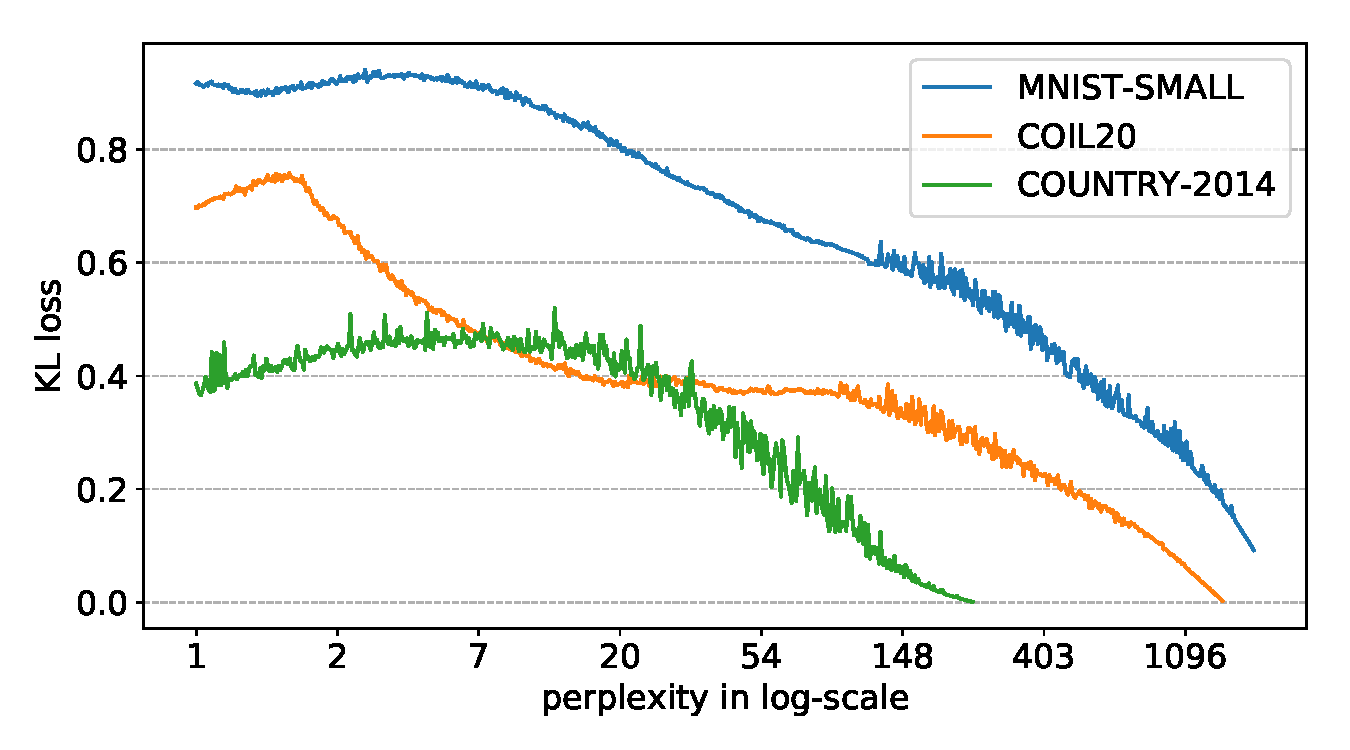
\includegraphics[width=0.95\linewidth]{klloss_all}
    \caption{For three different datasets, the KL loss tends to decrease when the perplexity increases. Note that the values of KL loss across different datasets are not comparable.}
    \label{fig:klloss}
\end{figure}

In practice, users have to carefully choose a hard-to-understand perplexity to obtain a good embedding result.
Even though this process requires an expertise in machine learning, it is often tedious and error-prone.
Our idea is to let users suggest \emph{how close instances have to be in the visualization} by using constraints, in order to propose the most suitable visualization for them.

Few papers in the literature attempt to derive the best perplexity automatically.
Strickert~\cite{strickert2012} evaluates the degree of neighborhood P*, instead of P, by using a given pairwise score matrix S. For each instance $i$ in ${\bf S}$, all other instances $j$ are ranked and {P*}$_{ij}$ is computed with respect to the ranking position of each instance $j$ in ${\bf S}_i$. However, this solution is not suitable when the matrix ${\bf S}$ is not provided.
Lee et al.~\cite{lee2014} use a multi-scale approach by considering, and averaging, all neighborhood sizes. Despite providing visualizations by bypassing the perplexity selection problem, Lee et al. do not offer a solution for the selection problem itself.
On the contrary, Cao and Wang~\cite{cao2017automatic} select the perplexity that minimizes the modified \emph{Bayesian Information Criteria} (\emph{BIC}):
\begin{equation}
S(\textit{perplexity}) = 2KL(P||Q) + \log(n)\frac{\textit{perplexity}}{n},
\end{equation}
where $KL(P||Q)$ is the same KL loss as Eq.~\ref{eq:KL} and $n$ is the number of instances.
Their approach is validated with user-based experiments by comparing the automatically selected visualization to the ones selected by users. They obtain resultant perplexities very close to the user consensus for three datasets.


\subsection{Automatic Hyperparameter Tuning with Bayesian Optimization}

The machine learning methods in general are controlled by one or many hyperparameters.
To use these methods efficiently, it requires a lot of skill to set hyperparameters.
The efficiency of a method is usually evaluated by a score,
e.g., F1-score for classification task, V-Measure score for clustering task or
visualization quality metric for DR task.
The goal is to jointy tune the ensemble of hyperparameters to
make the model output the highest score.
Trial-and-error method is typically used to test several common combinations of the parameters
but it is not a systematic way to tune the hyperparameters.

One common approach to solve this problem is naive grid search.
By making a list of discrete values for each hyperparameter,
we can try to evaluate all possible combinations.
The parameter space growns exponentially w.r.t. the number of hyperparameters
and the number of values for each one.
A better approach is random search \cite{bergstra2011algorithms}, in which we sample randomly the combinations.
From the list of alternative values for the hyper-parameters,
pick randomly one value for each hyper-parameter to create one combination.
But there are some hyper-parameters which have large effect and others which have no effect.
If we move along the axes of the no-effect hyperparameters, we do not learn at all.
Thus the question is how to jointly tune many hyperparameters at the same time
with as few evaluations as possible.
Bayesian optimization (BayOpt) is an anwser to our question.
We first explain the BayOpt approach in general, then explain how it fits to the hyperparameter tuning problem.

BayOpt is a strategy for finding the extremum (minimum or maximum) of an objective function $f$~\cite{mockus1975on}.
The objective function can be any complex non-convex blackbox function which does not have closed-form expression or its derivative is not accessible.
Thus finding directly the extremum of this kind of function is impossible.
However, we can observe the function values (possibly noisy) for some sampled input values.
The goal of BayOpt is not to approximate the unknown objective function $f$ but instead
estimate its extremum (generally speaking, its maximum) from the ensemble of observations
in form of pair of input sample $x$ and function values $f(x)$.

Let define $f(x_i)$ as the observation of the target function for the $i^{th}$ sample $x_i$.
BayOpt constructs a statistical model describing the relationship between
the tuning hypyerparamters and the target function.

NEED REVIEW: Bayesian model-based optimization is intuitive: choose the next input values to evaluate based on the past results to concentrate the search on more promising values.

BayOpt has been applied successfully to the problem of hyperparameters tuning \cite{snoek2012practical} or experimental design / randomized experiments \cite{letham2019constrained}.
We can consider the unknown objective function is our target function (score function) for all combinations of the hyperparameters.
Since we can not evaluate all combinations of the hyperparameters,
the target function is obviously unknown.
The goal is thus to find a best combination that maximize the target function.

\vspace{8pt} \par
TODO:

Discuss: BayOpt can be applied to the BIC-based score~\cite{cao2017automatic}.
However this score has two disavantages:
(1) it is tied to the loss function of t-SNE.
(2) it works only with one hyperparameter (perplexity of t-SNE), and thus can not be generalized for other DR methods.
Our proposed method can do better.



%%%%%%%%%%%%%%%%%%%%%%%%%%%%%%%%%%%%%%%%%%%%%%%%%%%%%%%%%%%%%%%%%%%%%%%%%%%%%%
\section{Constraint Preserving Score}

\subsection{Visual Definition of User Pairwise Constraints}

Since humans are capable of well distinguishing similar and dissimilar high-dimensional objects with prior knowledge (e.g. comparing countries only by their name, compare images by the visual features such as the shape, color, objects on image, etc.), they can naturally express their cognitive requirements by defining several links between instances.
In Fig.~\ref{fig:ml_cl_examples}, several examples are provided of similar-links that can be formed between objects between very similar objects under different point of view while the dissimilar-links would be formed between objects of different shapes.

\begin{figure}
    \centering
    \begin{subfigure}[c]{0.48\linewidth}
        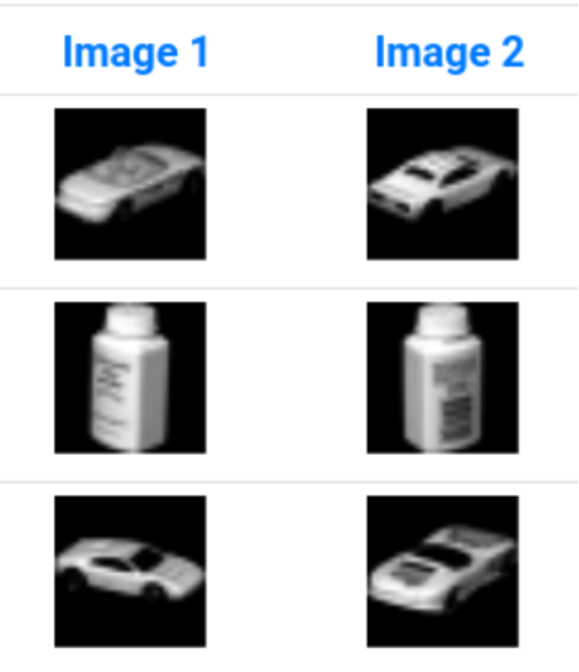
\includegraphics[width=\textwidth]{ml_examples}
        \caption{Similar-link constraints.}
    \end{subfigure}
    \begin{subfigure}[c]{0.48\linewidth}
        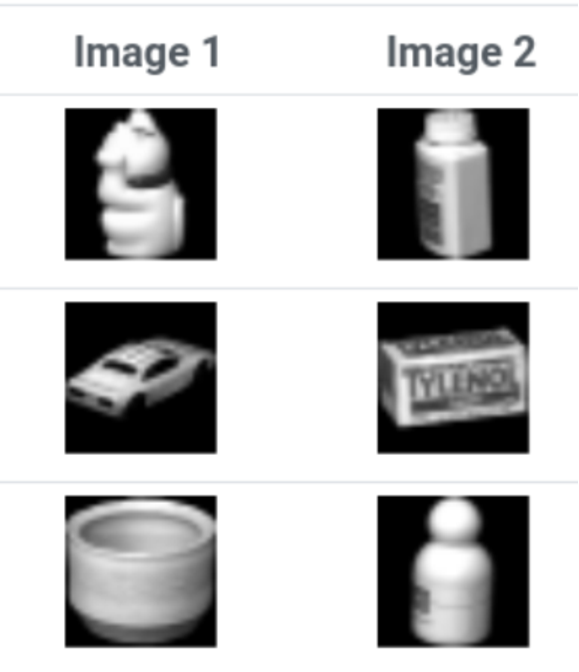
\includegraphics[width=\textwidth]{cl_examples}
        \caption{Dissimilar-link constraints.}
    \end{subfigure}
    \caption{Examples of similar-link and dissimilar-link constraints between pairs of images from COIL20 dataset (a dataset of 20 object captures under many different vantage points).}
    \label{fig:ml_cl_examples}
\end{figure}

Our method is based on the following hypothesis: an embedding is said to be good if it accurately represents the high-dimensional data and satisfies the user constraints. The pairwise constraints can then be used as a criterion to fit the user requirements.
Our method frees users from manually selecting the hyperparameter of $t$-SNE and provides a good quality embedding while preserving their predefined constraints.
To prove the reliability of this hypothesis, we transform the pairwise constraints to a quantitative score (defined in Section~\ref{subsec:s_score}) and compare it with several embedding quality metrics (presented in Section~\ref{subsec:metric}).

TODO:

+ Explain that  we use the auto-generated pairwise constraints when having labels.

+ We can ask the user to label a small proportion of labels in order to construct the pairwise constraints, or the user can select the constraints manually.


\subsection{Quantifying the User Constraints}\label{subsec:s_score}
Given an embedding result and a set of user pairwise constraints, our method outputs a score measuring how well the pairwise constraints are preserved in the output embedding, called \emph{constraint-preserving score} $S$.

\subsubsection*{Constraint measurement}
$t$-SNE uses the Student's $t$-distribution to encode the neighborhood information of the instances in the low dimensional space (see Eq.~\ref{eq:q_ij}).
We also use a $t$-distribution in the embedded space to quantify the user constraints preservation.
Let us denote the embedding result of $t$-SNE ${Y} = \{{y_i}\}$, a set of similar-links $\mathcal{M}$ and a set of dissimilar-links $\mathcal{C}$. The number of similar-link and dissimilar-link constraints are denoted by $|\mathcal{M}|$ and $|\mathcal{C}|$, respectively.
For a constrained pair $(i, j)$, the probability of $i$ and $j$ being neighbors is defined as
\begin{equation}\label{equ:q_link}
    q_{ij} = \frac
    { ( 1 + || y_i - y_j ||^2 )^{-1} }
    { \sum_{k \neq l} { ( 1 + ||y_k - y_l||^2 )^{-1} } }.
\end{equation}
The points connected by a similar-link constraint are considered as neighbors and should be close together.
The constrained points in a dissimilar-link should stay apart since they can not be neighbors of each other.
Therefore, for each similar-link $(i,j) \in \mathcal{M}$, $q_{ij}$ should be high and inversely, $q_{ij}$ is expected to be low for each dissimilar-link $(i,j) \in \mathcal{C}$.

\subsubsection*{Constraint-preserving score for similar-links}
The amount of similar-link information preserved in a given embedding is measured as a log-likelihood of the joint distribution of $q_{i j}$ over all similar-links $(i, j) \in \mathcal{M}$:
\begin{equation}
S_{\mathcal{M}} = \frac{1}{|\mathcal{M}|} \log \prod_{(i,j) \in \mathcal{M}} q_{ij}
                = \frac{1}{|\mathcal{M}|} \sum_{(i,j) \in \mathcal{M}} \log q_{ij}.
\end{equation}
If all pairs connected by similar-links are placed close together, the log-likelihood is high and $S_{\mathcal{M}}$ is maximized.

\subsubsection*{Constraint-preserving score for dissimilar-links}
In contrast to similar-links, the probability $q_{ij}$ for each dissimilar-link $(i,j) \in \mathcal{C}$ should be low, i.e. the log-likelihood over all dissimilar-link pairs ($\log \prod_{\mathcal{C}} q_{ij}$) has to be minimized. Or in other words, the negative log-likelihood over all dissimilar-link constraints should be maximized. The constraint-preserving score for a set of dissimilar-links $\mathcal{C}$ is defined as
\begin{equation}
S_{\mathcal{C}} = -\frac{1}{|\mathcal{C}|} \log \prod_{(i,j) \in \mathcal{C}} q_{ij}
                = -\frac{1}{|\mathcal{C}|} \sum_{(i,j) \in \mathcal{C}} \log q_{ij}.
\end{equation}
By maximizing $S_{\mathcal{C}}$, the embedding that respects the best the dissimilar-link constraints is found.
Another way to measure how well a dissimilar-link $(i,j)$ is preserved is to use $1 - q_{ij}$. However, in practice, the value of $q_{ij}$ is very small, which means that $1 - q_{ij}$ is very close to one which makes the log-likelihood of all dissimilar-links vanish.

\subsubsection*{Constraint-preserving score for similar-links and dissimilar-links}

\begin{figure}
    \centering
    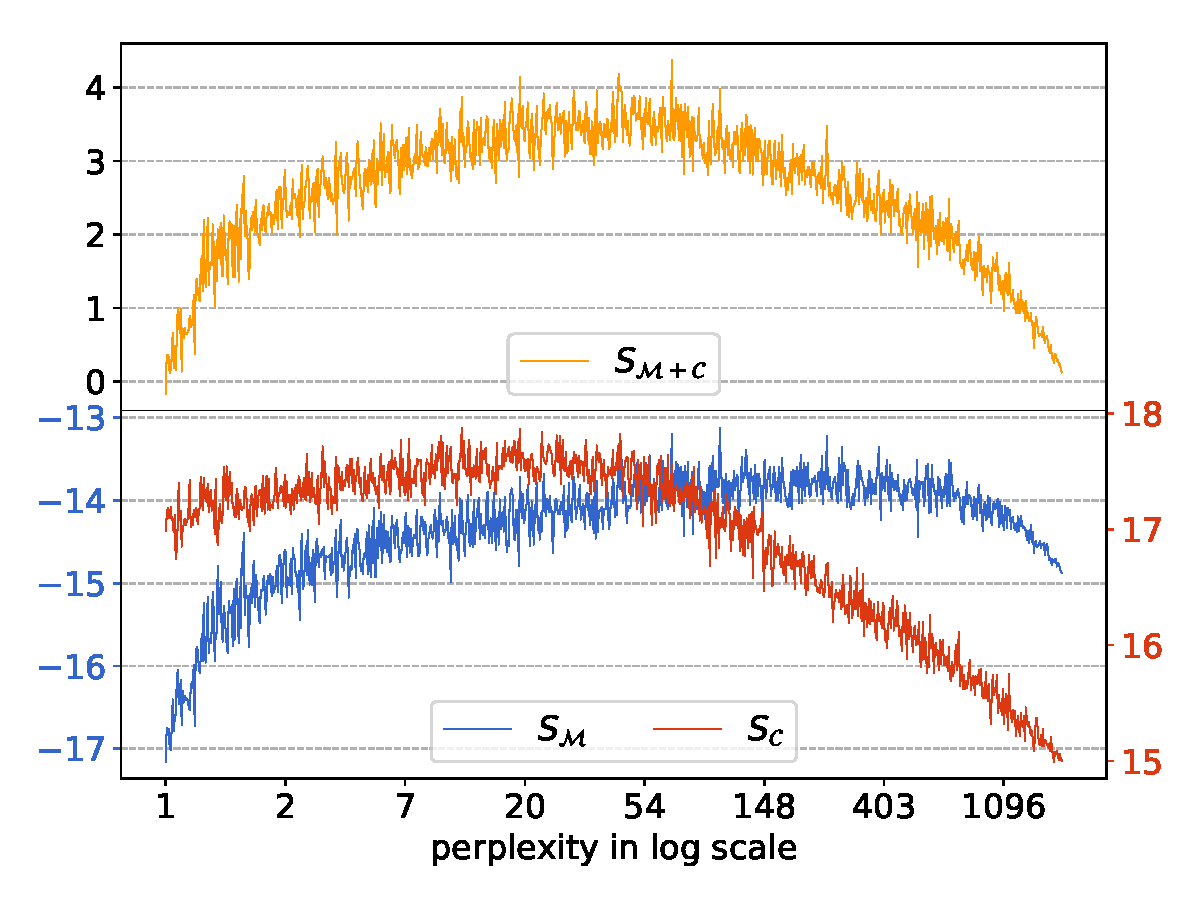
\includegraphics[width=0.85\linewidth]{s_scores_50}
    \caption{[TODO: Replace]Evolution of constraint-preserving scores $S_{\mathcal{M}+\mathcal{C}}$, $S_{\mathcal{M}}$ and $S_{\mathcal{C}}$ with 50 constraints for \emph{DIGITS} over different perplexities.}
    \label{fig:s_scores_mnist}
\end{figure}

The score over all similar-links and dissimilar-links can be maximized at the same time by defining the constraint-preserving score as a combination with equal contribution of both $S_{\mathcal{M}}$ and $S_{\mathcal{C}}$, i.e. $S_{\mathcal{M}+\mathcal{C}} = S_{\mathcal{M}} + S_{\mathcal{C}}$.

An embedding that retains as much as possible the constraint information is considered to have a good quality with respect to the user needs.
Based on these definitions, our method takes a set of user-defined pairwise constraints and searches among all embeddings created by different perplexities for one with maximal $S_{\mathcal{M}+\mathcal{C}}$.
Fig.~\ref{fig:s_scores_mnist} illustrates the contribution of $S_{\mathcal{M}}$ and $S_{\mathcal{C}}$ to the overall $S_{\mathcal{M}+\mathcal{C}}$ score for \emph{DIGITS} dataset with 50 auto-generated constraints (see Section~\ref{subsec:constraint_preparation} for details about the generation process).


%%%%%%%%%%%%%%%%%%%%%%%%%%%%%%%%%%%%%%%%%%%%%%%%%%%%%%%%%%%%%%%%%%%%%%%%%%%%%%
%%%%%%%%%%%%%%%%%%%%%%%%%%%%%%%%%%%%%%%%%%%%%%%%%%%%%%%%%%%%%%%%%%%
\section{Constraint-based Score as Target in Bayesian Optimization Approach}

+ Explain the internal step in BayOpt.
Can make use some figures Fig.~\ref{fig:bayopt5}, Fig.\ref{fig:bayopt10}.

\begin{figure}
\centering

    \begin{subfigure}[b]{0.5\textwidth}
        \centering
        \includegraphics[width=\textwidth]{{ucb_kappa5_COIL20_step5}.png}
        \caption{BayOpt after 5 steps.}\label{fig:bayopt5}
     \end{subfigure}
     \vfill

    \begin{subfigure}[b]{0.5\textwidth}
        \centering
        \includegraphics[width=\textwidth]{{ucb_kappa5_COIL20_step10}.png}
        \caption{BayOpt after 10 steps.}\label{fig:bayopt10}
    \end{subfigure}
    \vfill

    \begin{subfigure}[b]{0.5\textwidth}
        \centering
        \includegraphics[width=\textwidth]{{ucb_kappa5_COIL20_step15}.png}
        \caption{BayOpt after 15 steps.}\label{fig:bayopt10}
    \end{subfigure}

\caption{BayOpt in action (COIL20, tsne, ucb, kappa5)}\label{fig:bayopt_progress}
\end{figure}


+ Explain how the utility function are constructed and optimized, and answer why optimize the utility function (surrogate function), we can optimize at the same time the target function (the constraint-based score function).

+ Explain the exploitation-exploration trade-off in BayOpt (and estimate the number of times we need to try before reaching to the global maximum).

+ Show that BayOpt gives stable prediction (at least, the best range).
Demo with e.g., COIL20 or DIGITS, keep the same input constraint set,
change random seed for BayOpt, and get around the same prediction for the best range.

%%%%%%%%%%%%%%%%%%%%%%%%%%%%%%%%%%%%%%%%%%%%%%%%%%%%%%%%%%%%%%%%%%%%%%%%%%%%%%
\section{Experimental Results}

Present the dataset, the used pairwise constraint, the workflow as in the section 5.1, 5.2.

To present and analyze the results, we can present following points (but we still miss the evaluation).

(1) Optimal hyperparameters found by BayOpt w.r.t the constraint-based score:

+ BayOpt method for finding \verb|perplexity| param for t-SNE. (Case of 1 param to tune with t-SNE, Fig.~\ref{fig:tsne1}) (Done)
\begin{figure*}
\centering
\includegraphics[width=.8\textwidth]{{bo_summary_COIL20_tsne_ei}.png}
\caption{BayOpt with t-SNE with 1 param.}\label{fig:tsne1}
\end{figure*}

+ Add experiment with LargeVis. (TODO)

+ \st{BayOpt for finding n-neighbors param for UMAP. (Case of 1 param to tune with UMAP) (Done) } %Fig.~\ref{fig:umap1})
%% \begin{figure*}
%% \centering
%% \includegraphics[width=.6\textwidth]{{UMAP_ucb_kappa5_constraint1.0_DIGITS_step15}.png}
%% \caption{BayOpt with UMAP with 1 param.}\label{fig:umap1}
%% \end{figure*}

+ BayOpt for finding \verb|n_neighbors| and \verb|min_dist| params for UMAP. (Case of 2 params to tune with UMAP, Fig.~\ref{fig:umap2}) (Plan to do)
\begin{figure*}
\centering
\includegraphics[width=0.6\textwidth]{{objective_COIL20_umap}.png}
\caption{TODO: Produce a figure similar to this one with 2 params of umap.}\label{fig:umap2}
\end{figure*}


\begin{figure*}
     \centering
     \begin{subfigure}[b]{0.48\textwidth}
         \centering
         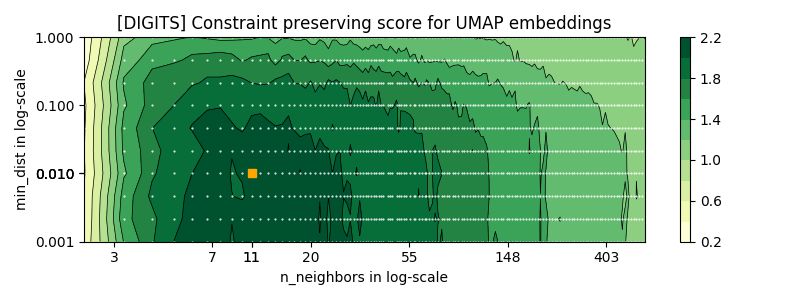
\includegraphics[width=\textwidth]{DIGITS_umap_qij_score}
         \caption{UMAP with DIGITS constraint score}
         \label{fig:s4}
     \end{subfigure}
     \hfill
     \begin{subfigure}[b]{0.48\textwidth}
         \centering
         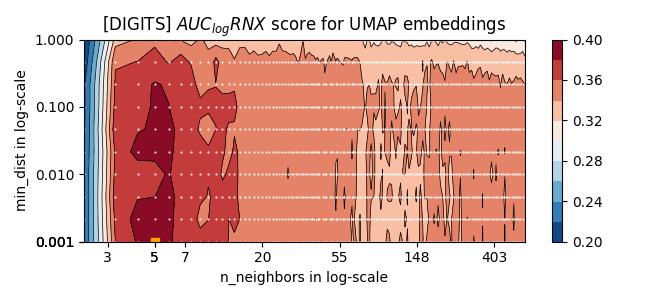
\includegraphics[width=\textwidth]{DIGITS_umap_auc_rnx}
         \caption{t-SNE with DIGITS John's score}
         \label{fig:s3}
     \end{subfigure}

     \vfill

    \begin{subfigure}[b]{0.48\textwidth}
         \centering
         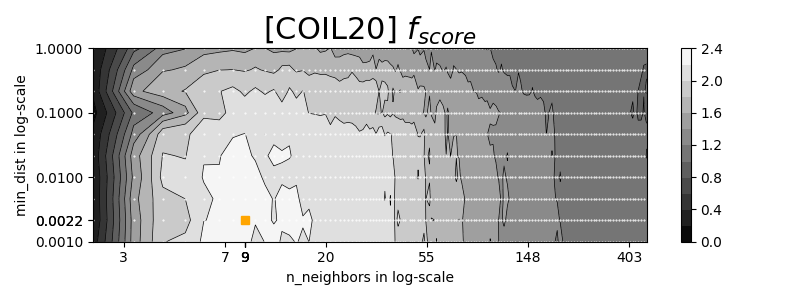
\includegraphics[width=\textwidth]{COIL20_umap_qij_score}
         \caption{UMAP with COIL20 constraint score}
         \label{fig:s4}
     \end{subfigure}
     \hfill
     \begin{subfigure}[b]{0.48\textwidth}
         \centering
         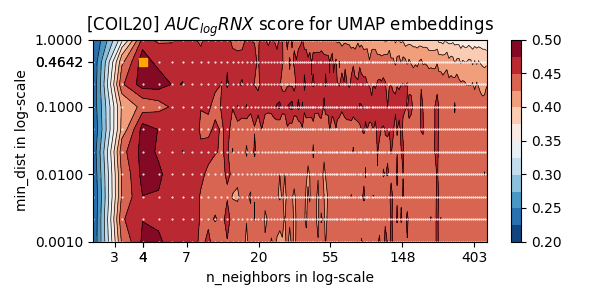
\includegraphics[width=\textwidth]{COIL20_umap_auc_rnx}
         \caption{t-SNE with COIL20 John's score}
         \label{fig:s3}
     \end{subfigure}
     \caption{BayOpt with UMAP(nneighbors, mindist)}
     \label{fig:umap2}
\end{figure*}

\vspace{8pt} \par
(2) Visualization of the violated constraints. (Doing, a draft version looks like
Fig.\ref{fig:viz-score})
We can analyze the explainability of the score / the visual assessment of the quality.

\begin{figure}
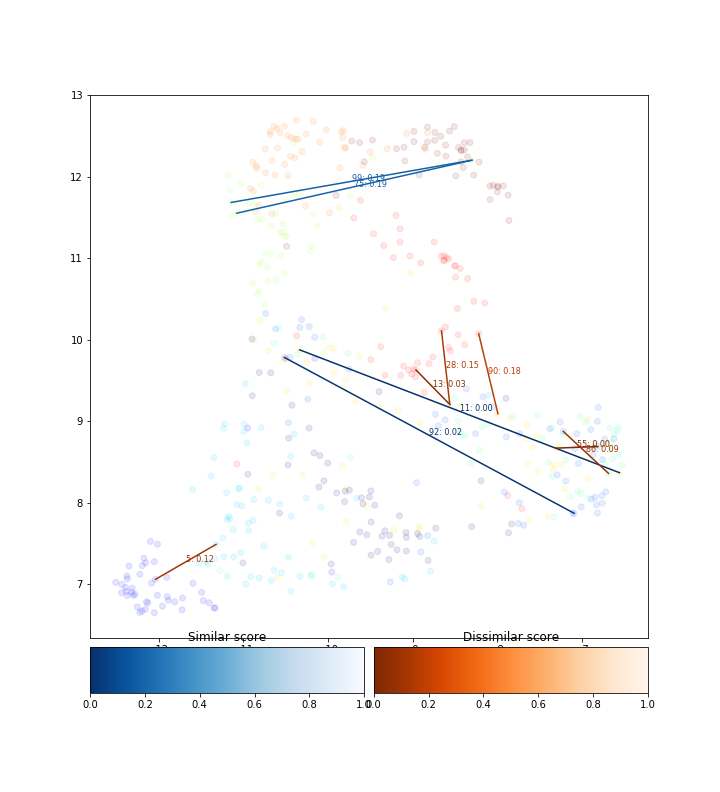
\includegraphics[scale=0.3]{umap_vis_score.png}
\caption{TODO Visualize the constraint score (of the violated links).}\label{fig:viz-score}
\end{figure}


\vspace{9pt} \par
(3) Analyse the characteristics of the constraint-based score.

+ Keep the section 6.2:

\hspace{10pt }- Must-link score agrees with CCA score (Fig~\ref{fig:sml}).
\begin{figure}
\centering
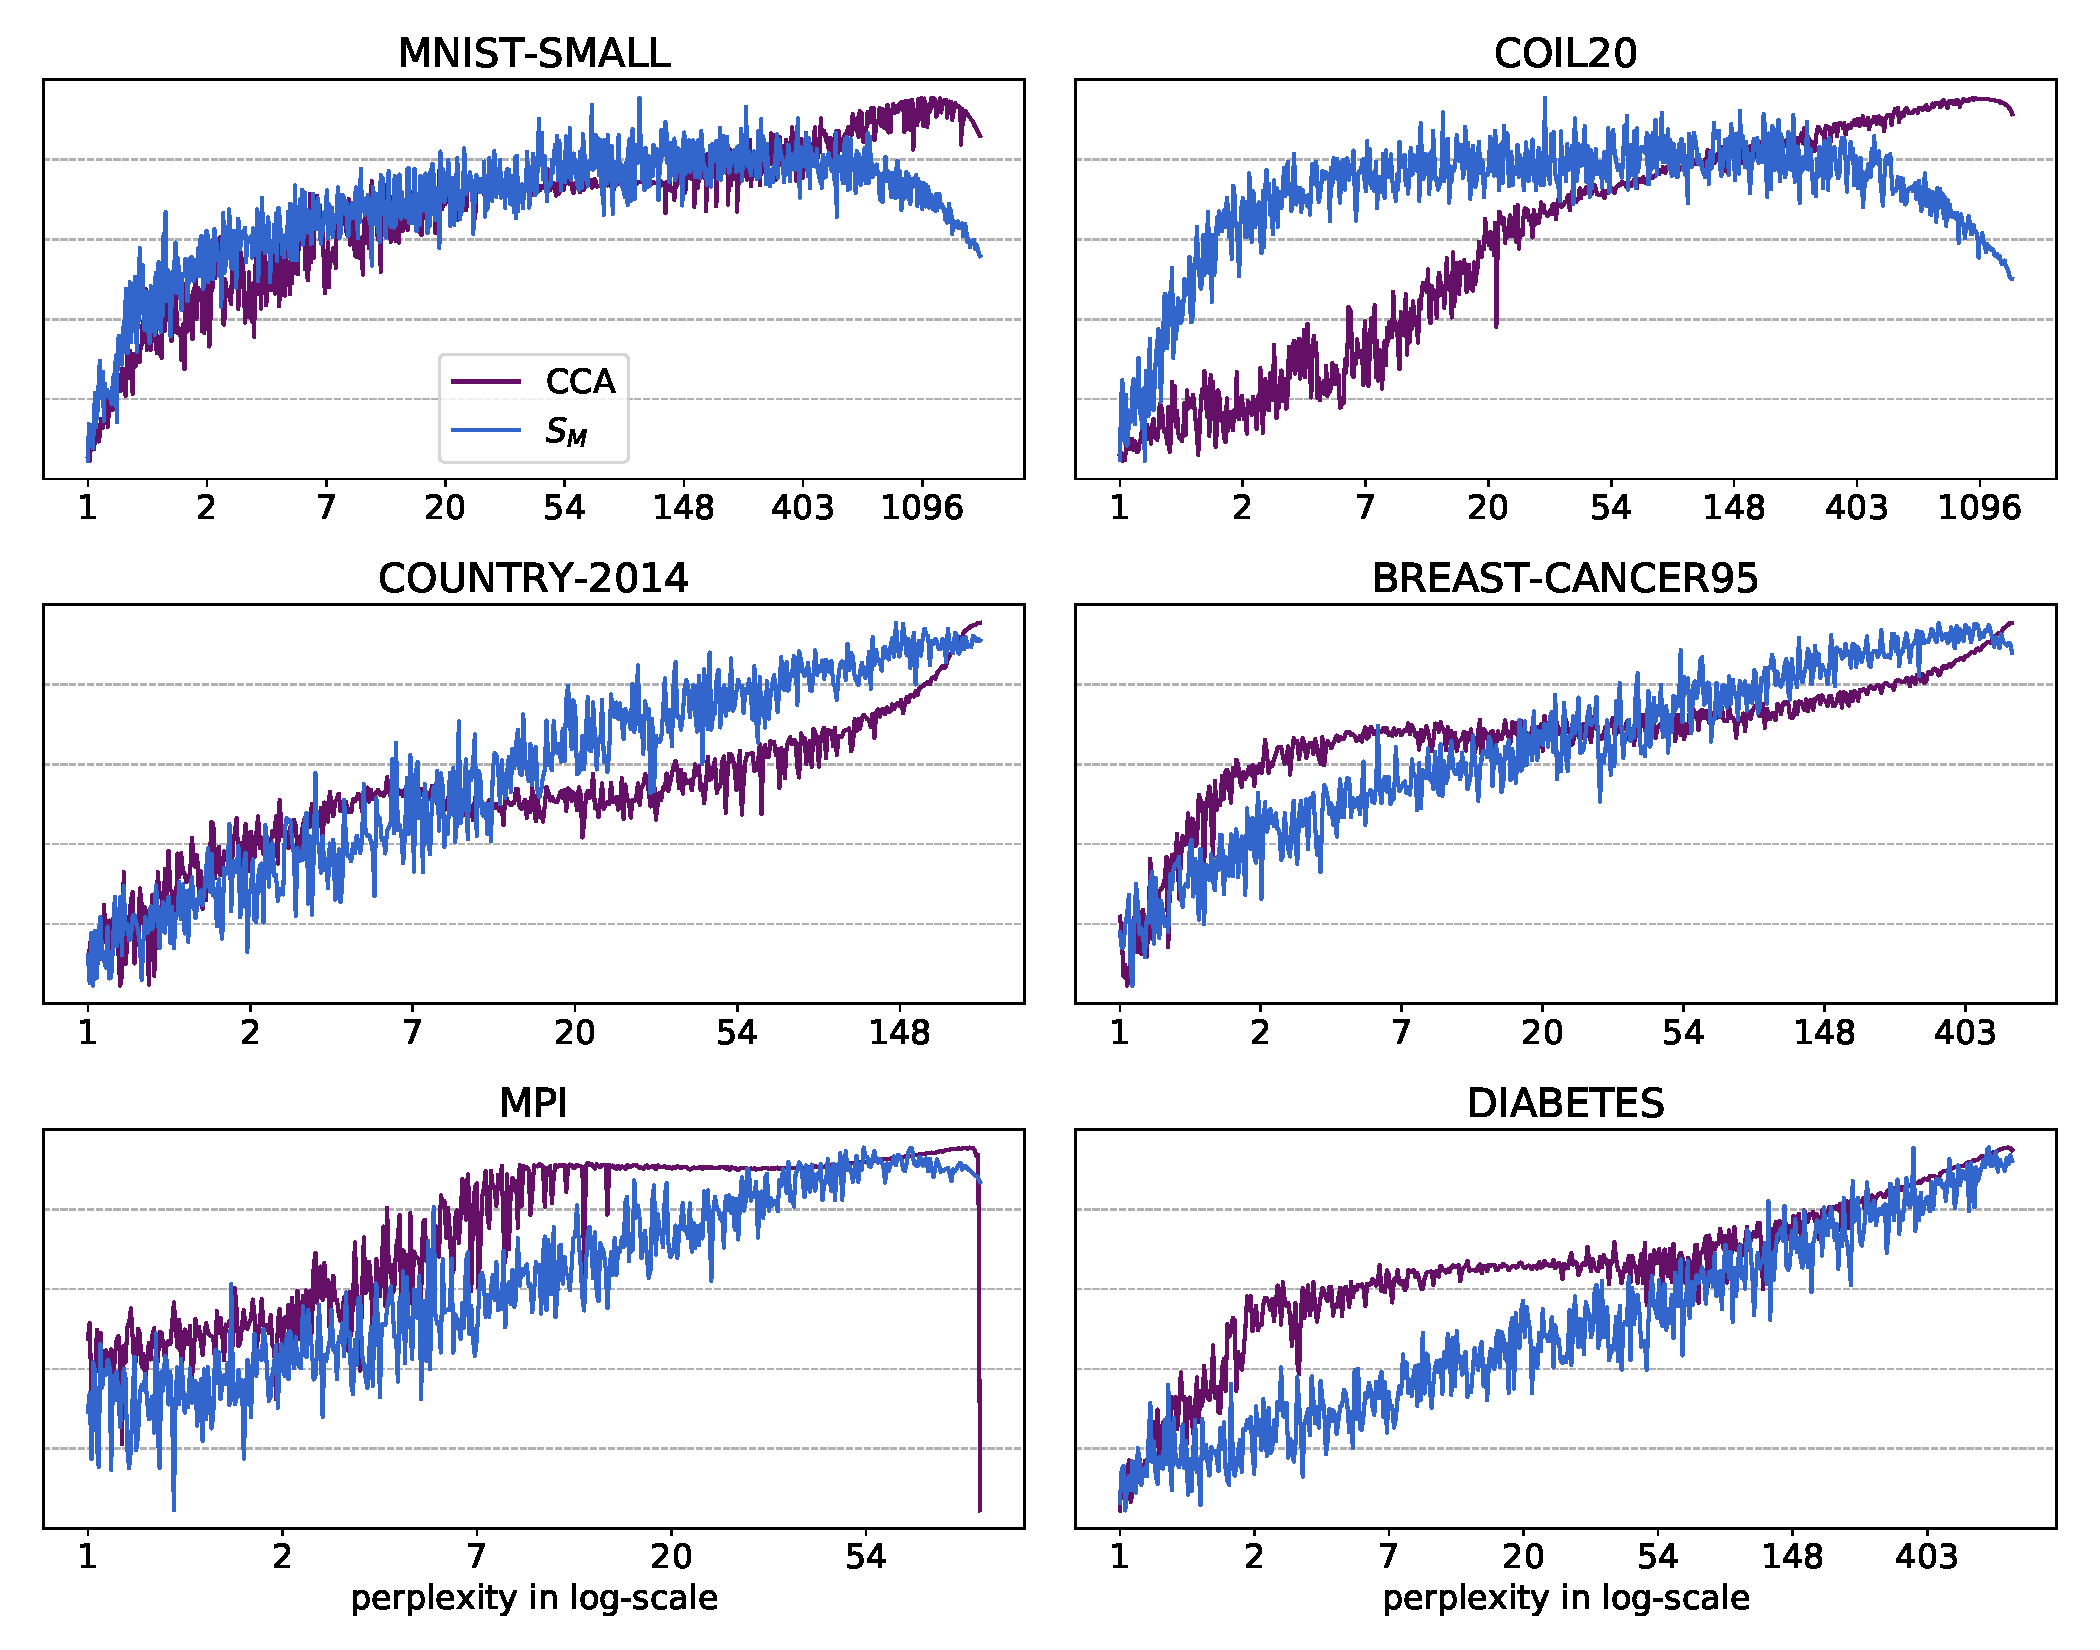
\includegraphics[scale=0.25]{sml_cca_50.pdf}
\caption{Must-link score agrees with CCA score.}\label{fig:sml}
\end{figure}

\hspace{10pt }- Cannot-link score agrees with BIC-based score (Fig.~\ref{fig:scl}).
\begin{figure}
\centering
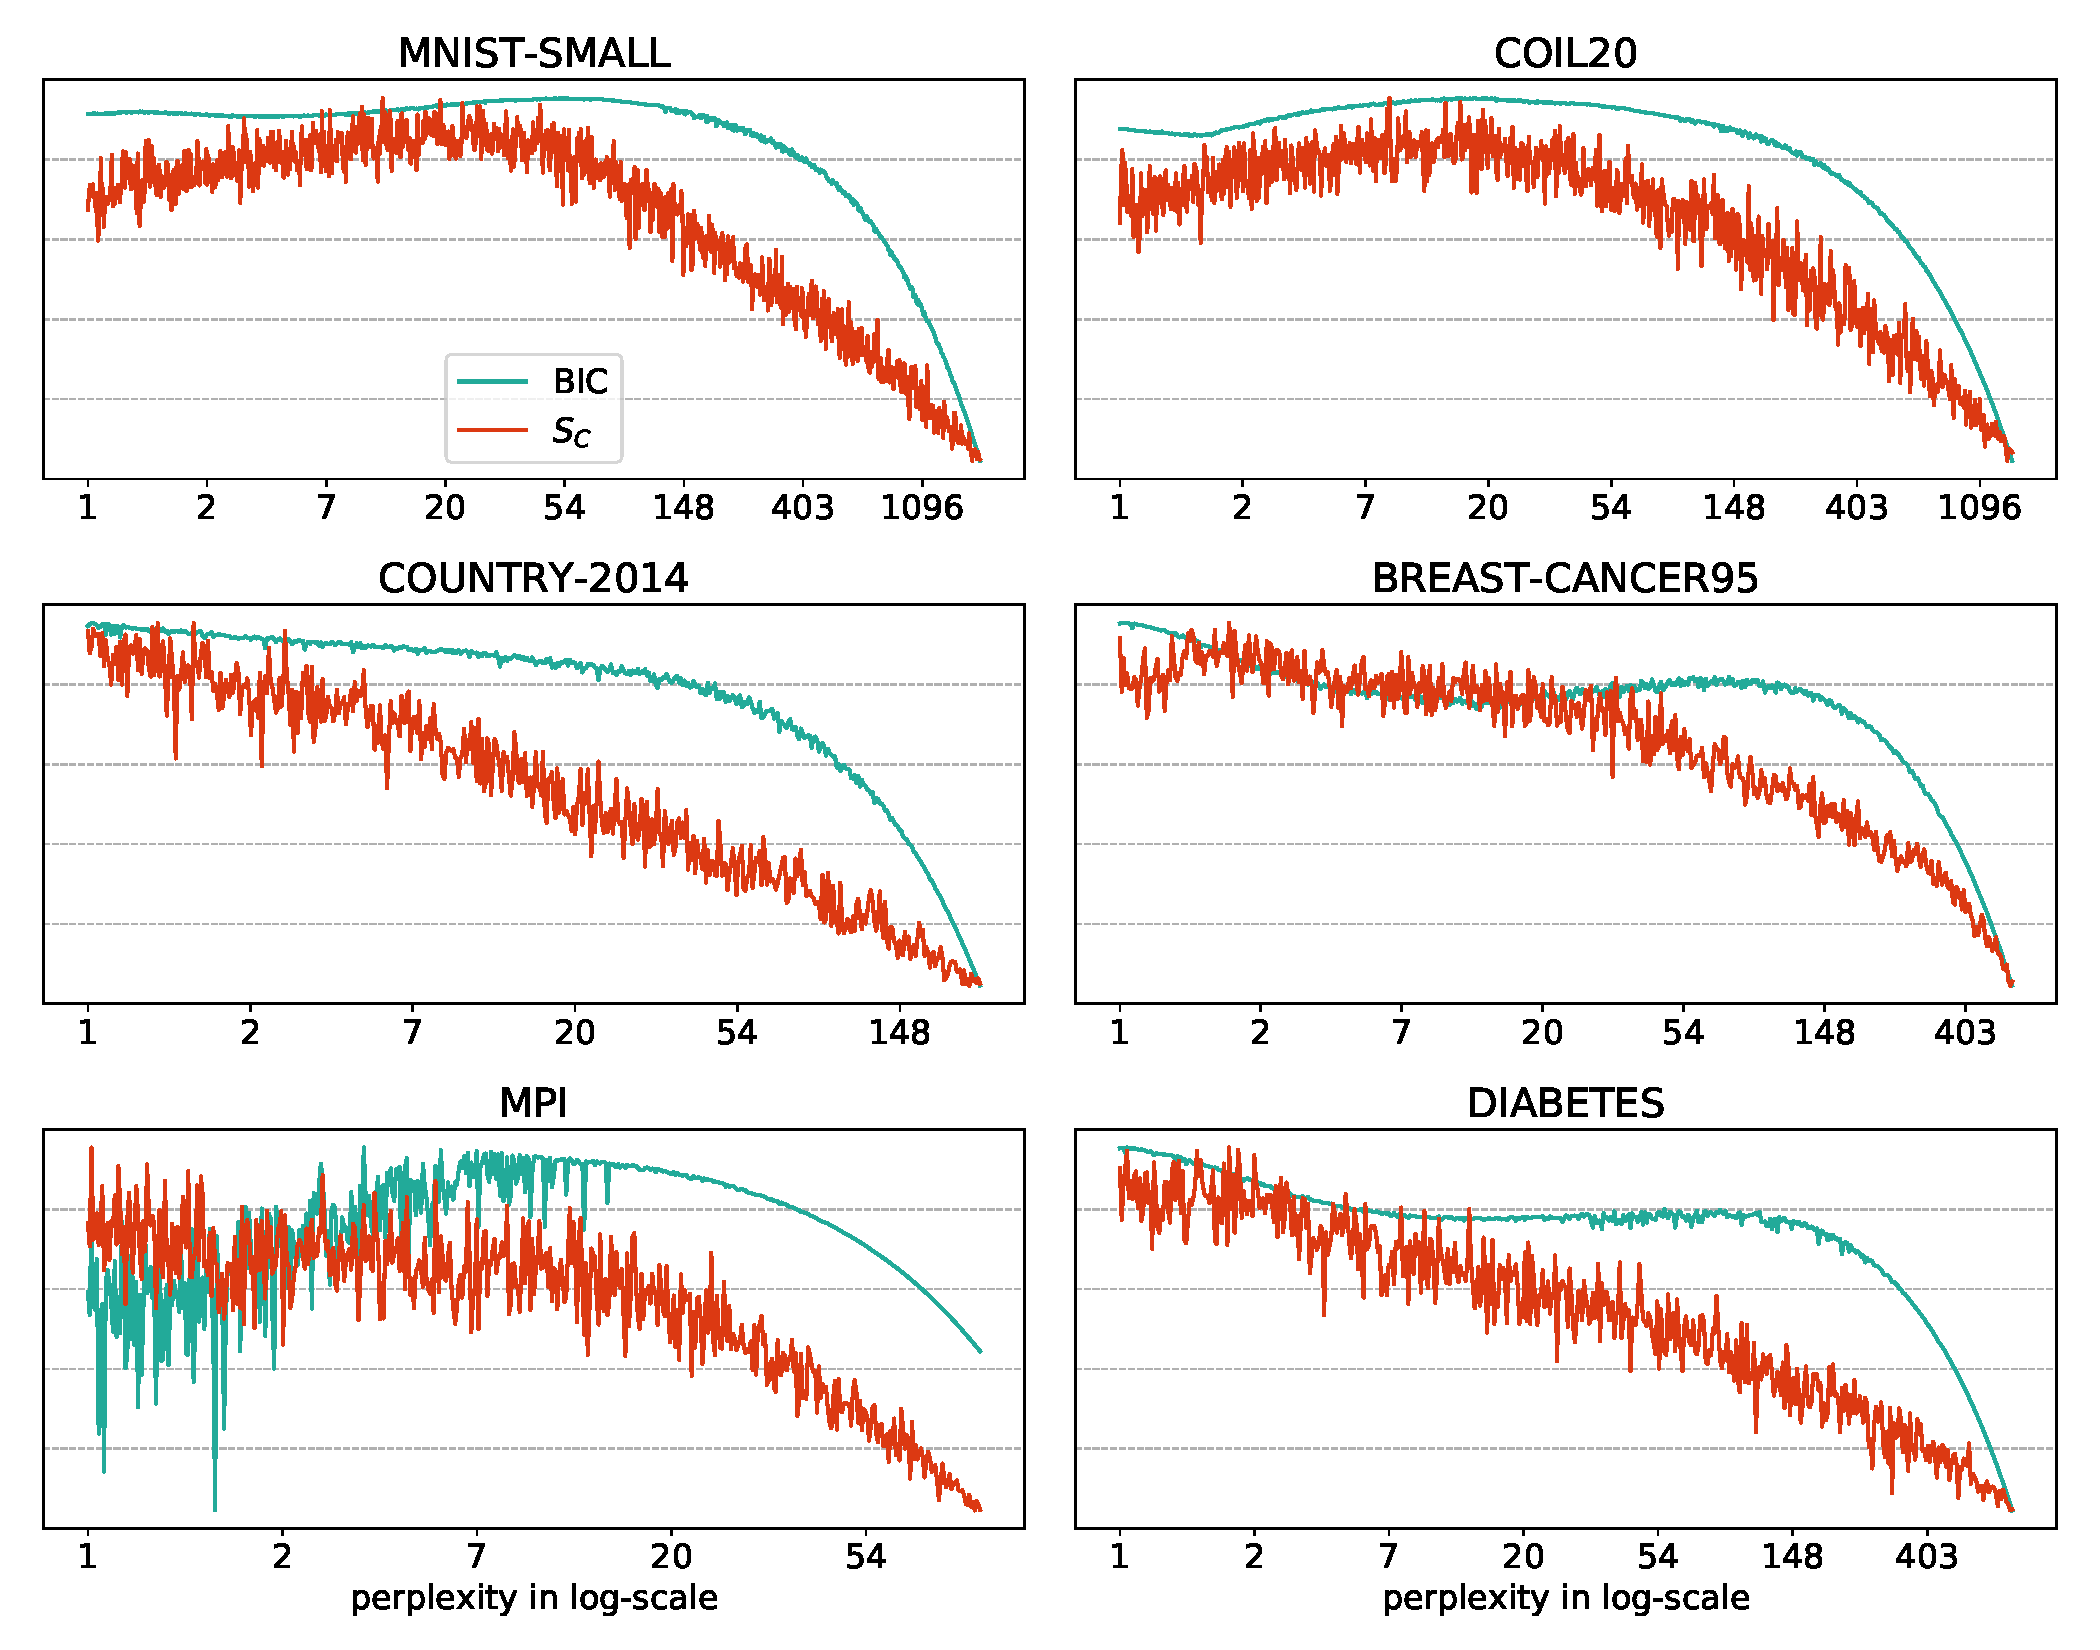
\includegraphics[scale=0.25]{scl_bic_50.pdf}
\caption{Cannot-link score agrees with BIC-based score.}\label{fig:scl}
\end{figure}

\hspace{10pt }- ML+CL agrees with AUC\_RNX score (Fig.~\ref{fig:sall}).
\begin{figure}
\centering
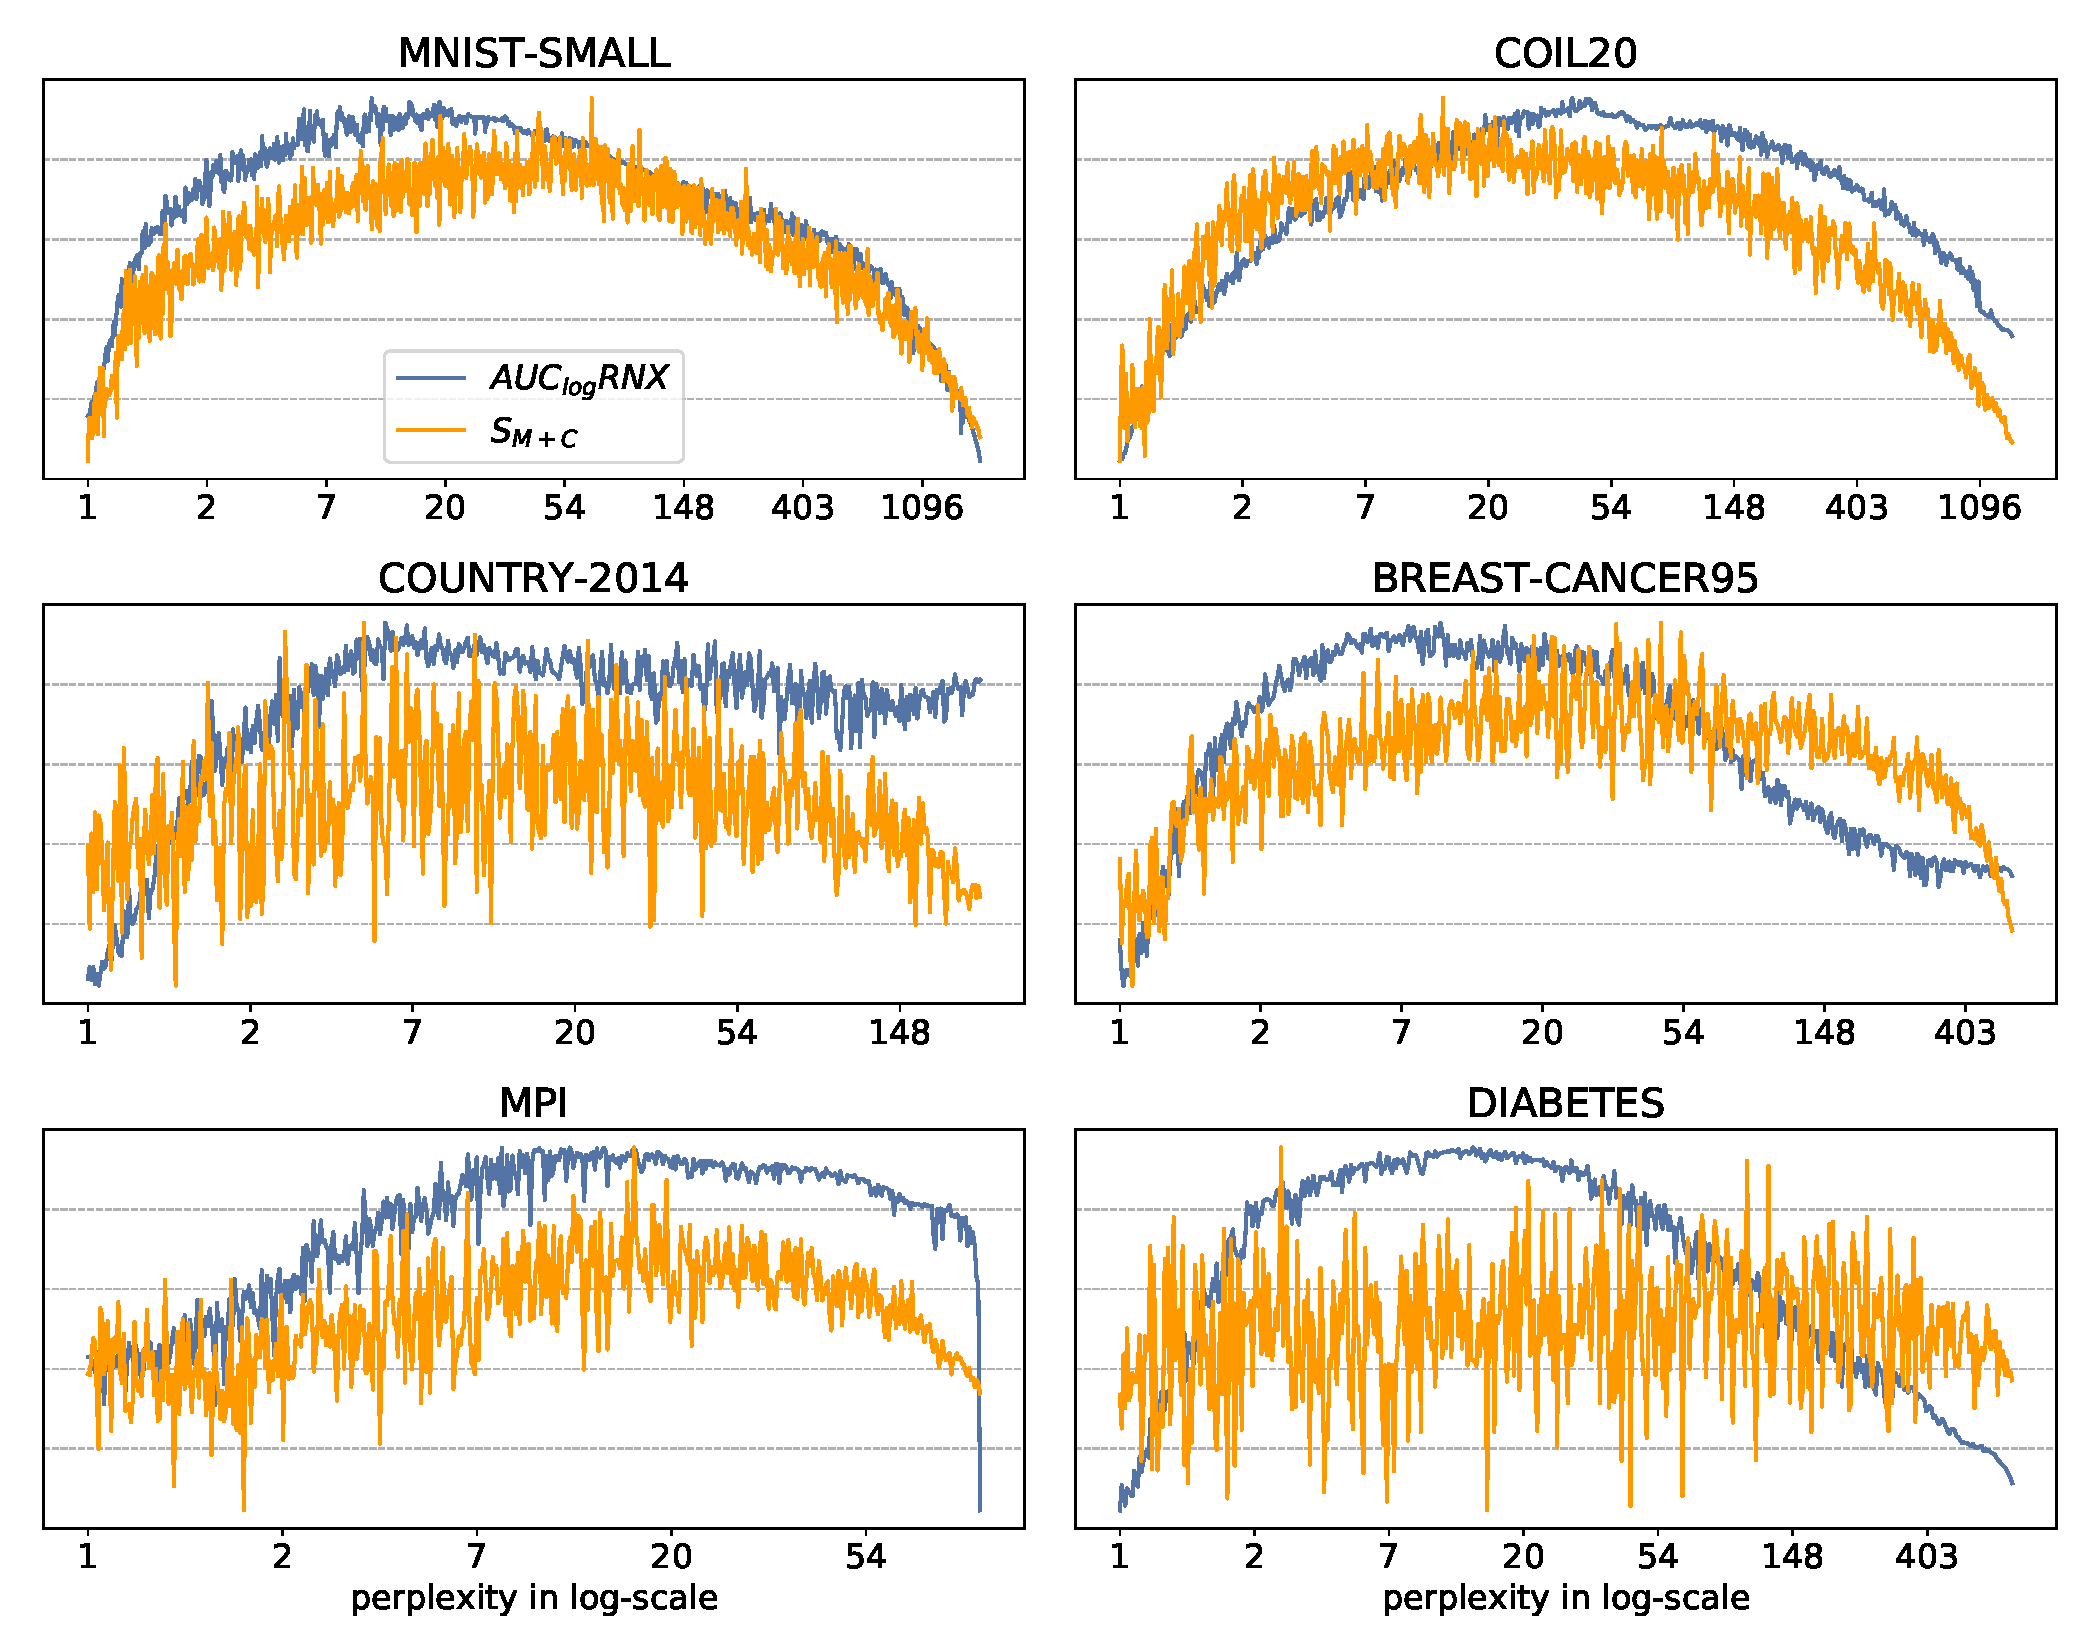
\includegraphics[scale=0.25]{sall_auc_50.pdf}
\caption{ML+CL agrees with AUC\_RNX score.}\label{fig:sall}
\end{figure}

\vspace{8pt} \par
+ Variance / Stability of the score: analyze Fig.~\ref{fig:score_stability} and explain how BayOpt approach can take into account the variance (uncertainty) of the score.

\begin{figure*}
     \centering
     \begin{subfigure}[b]{0.32\textwidth}
         \centering
         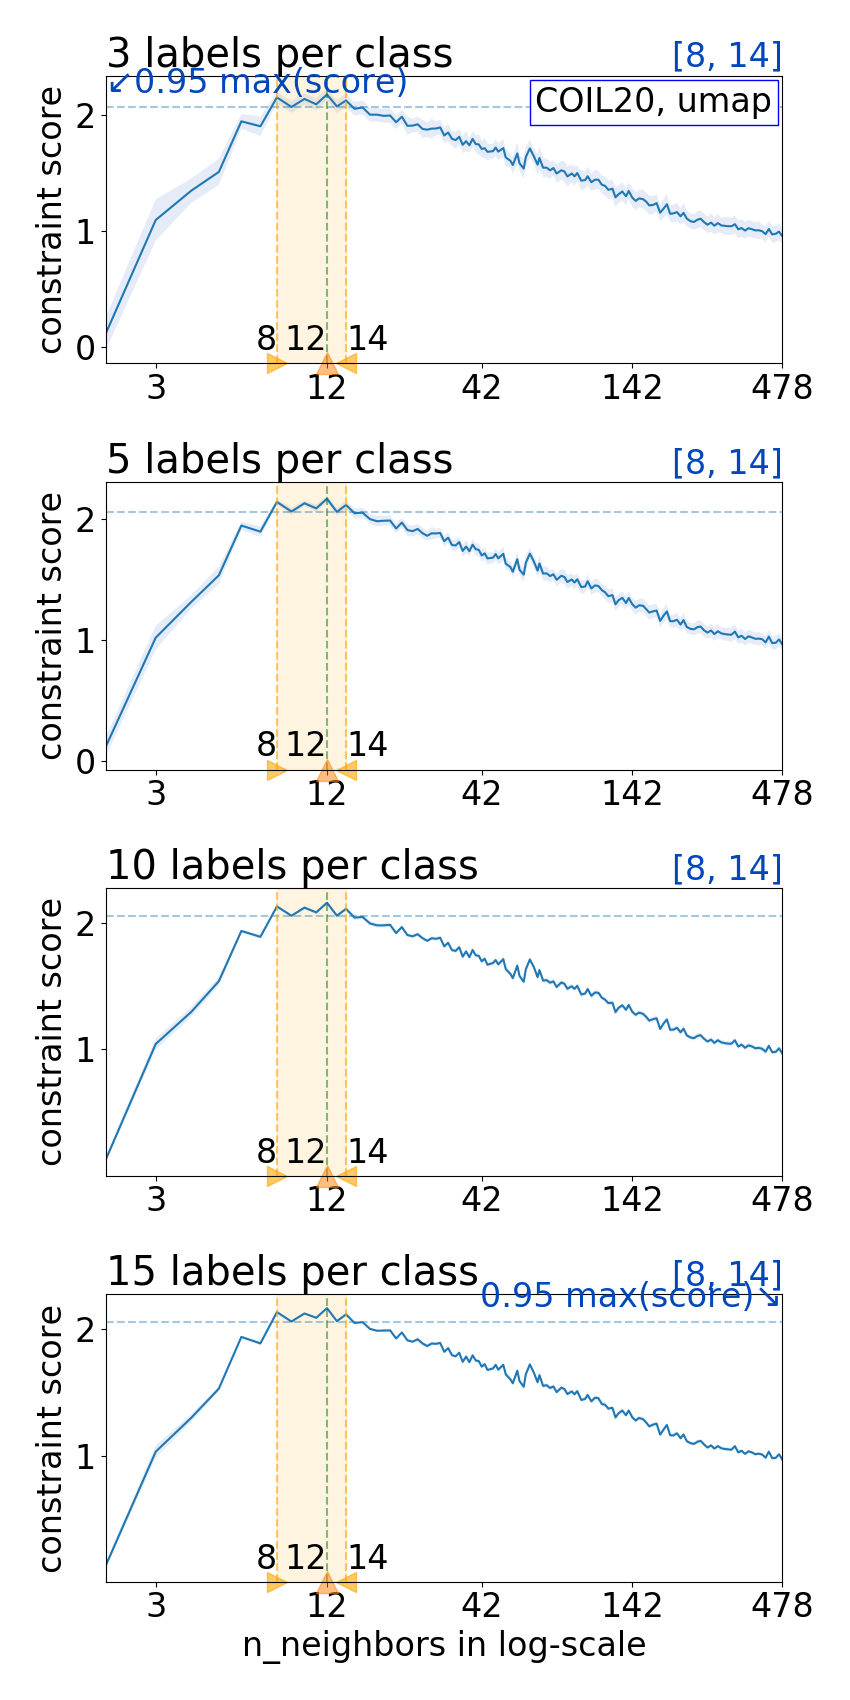
\includegraphics[width=\textwidth]{COIL20_umap_scores}
         \caption{UMAP with COIL20}
         \label{fig:s4}
     \end{subfigure}
     \hfill
     \begin{subfigure}[b]{0.32\textwidth}
         \centering
         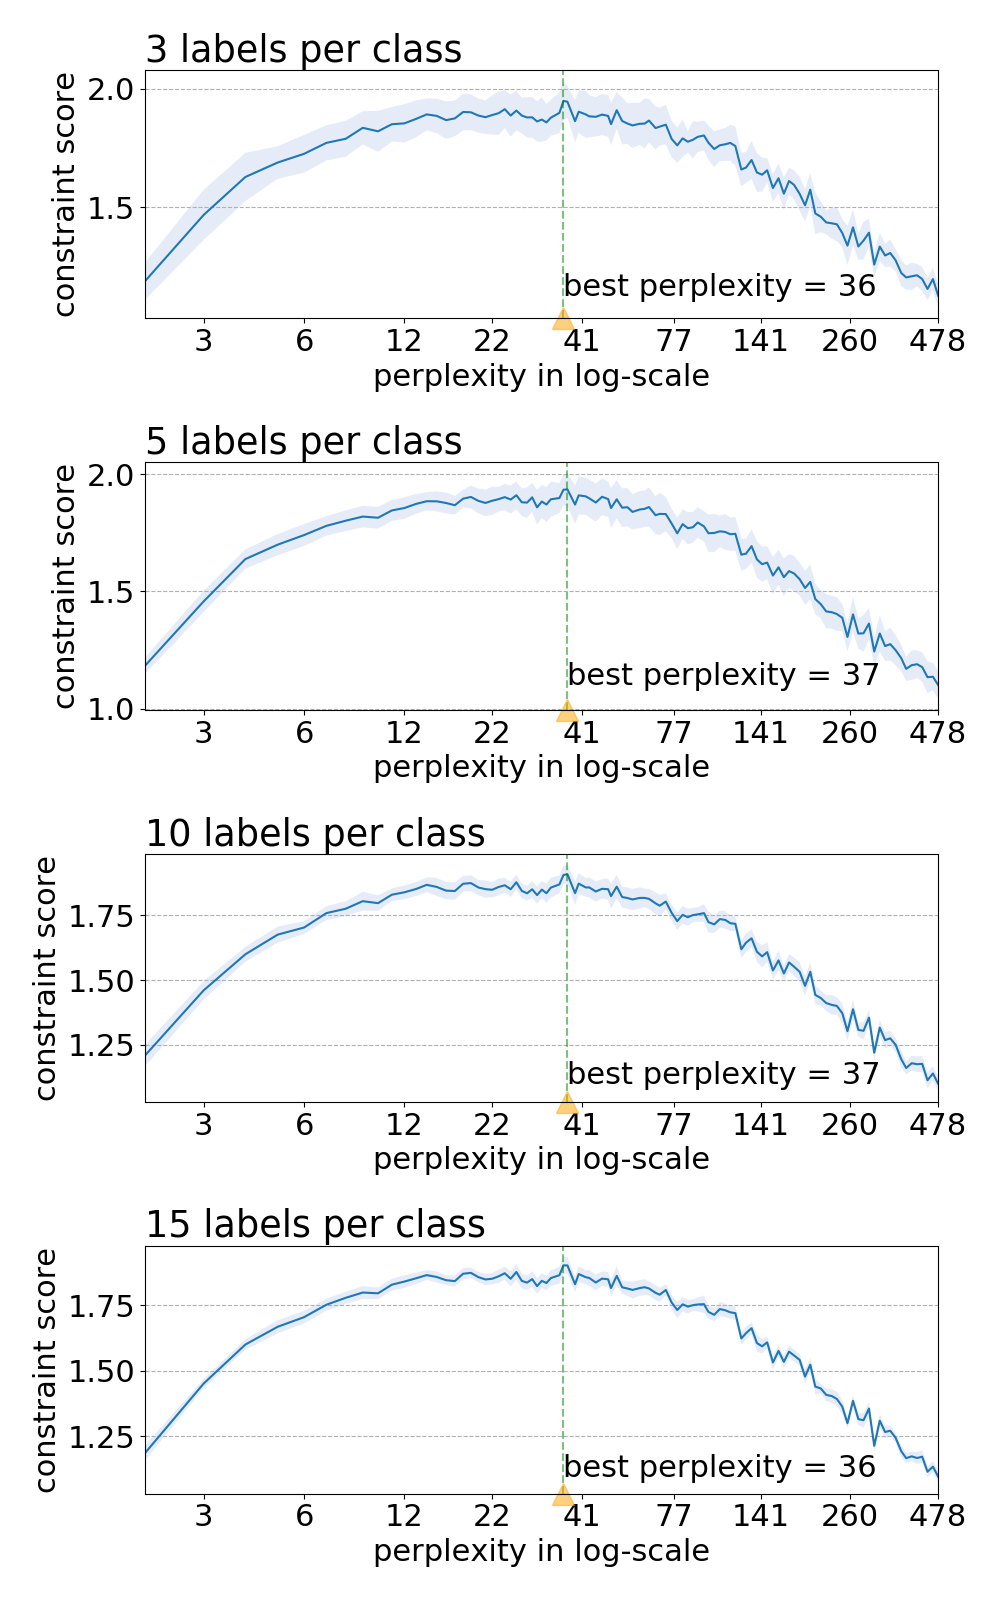
\includegraphics[width=\textwidth]{COIL20_tsne_scores}
         \caption{t-SNE with COIL20}
         \label{fig:s3}
     \end{subfigure}
     \hfill
     \begin{subfigure}[b]{0.32\textwidth}
         \centering
         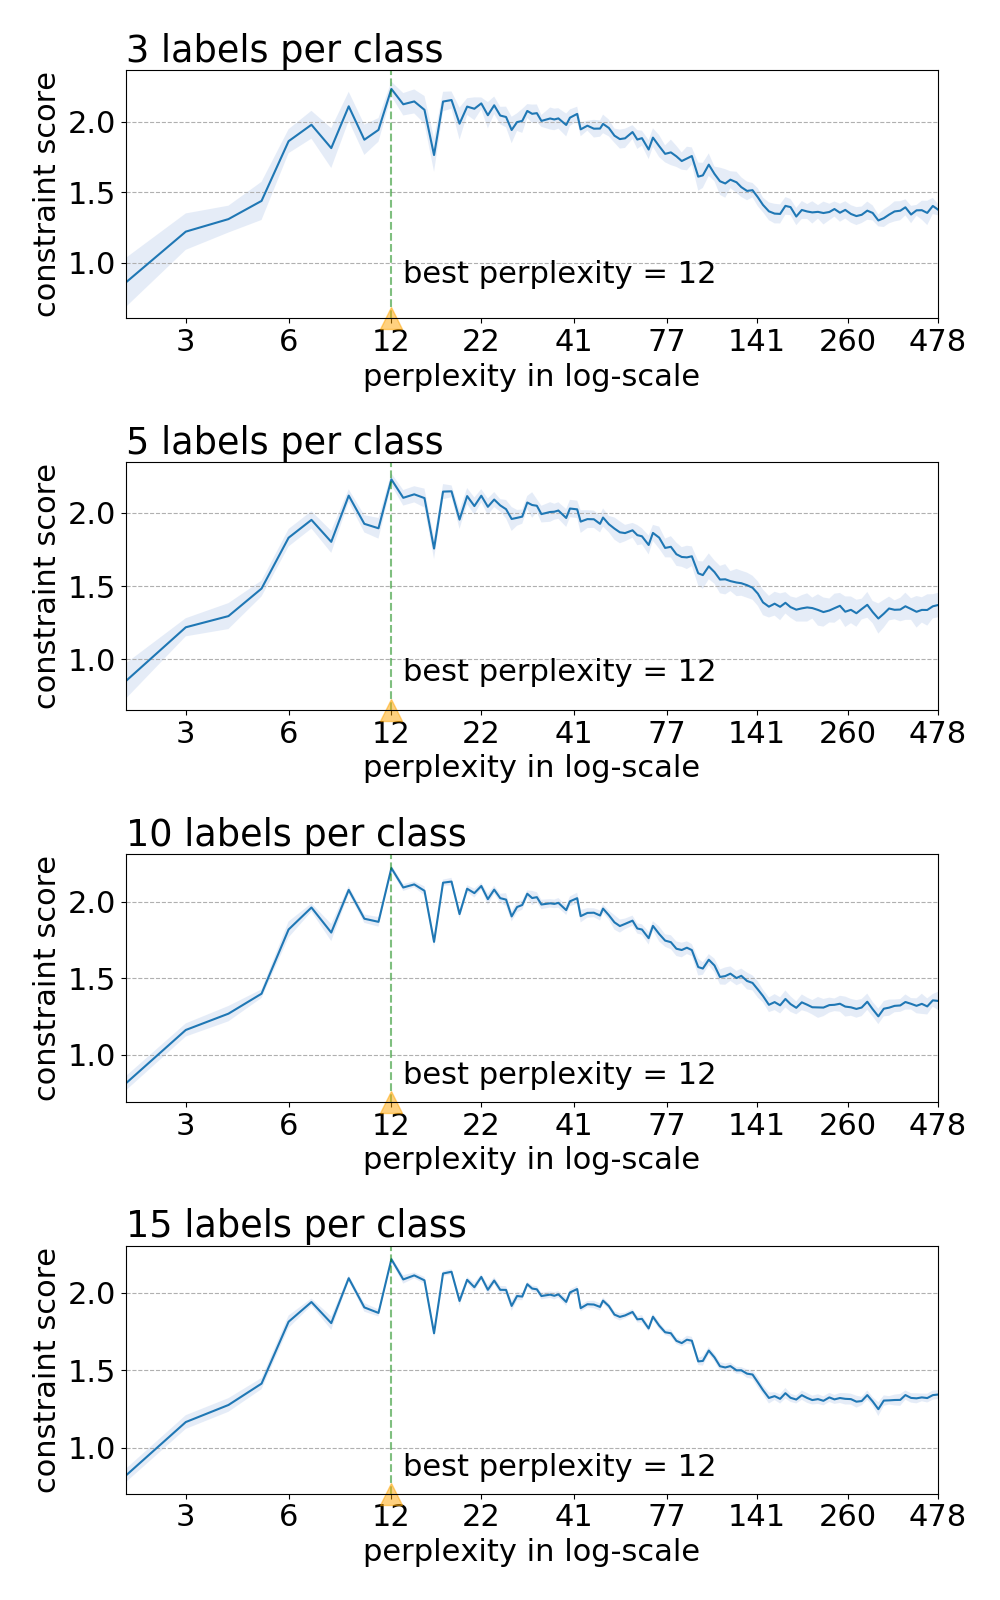
\includegraphics[width=\textwidth]{COIL20_largevis_scores}
         \caption{LargeVis with COIL20}
         \label{fig:s4}
     \end{subfigure}

     \vfill

     \begin{subfigure}[b]{0.32\textwidth}
         \centering
         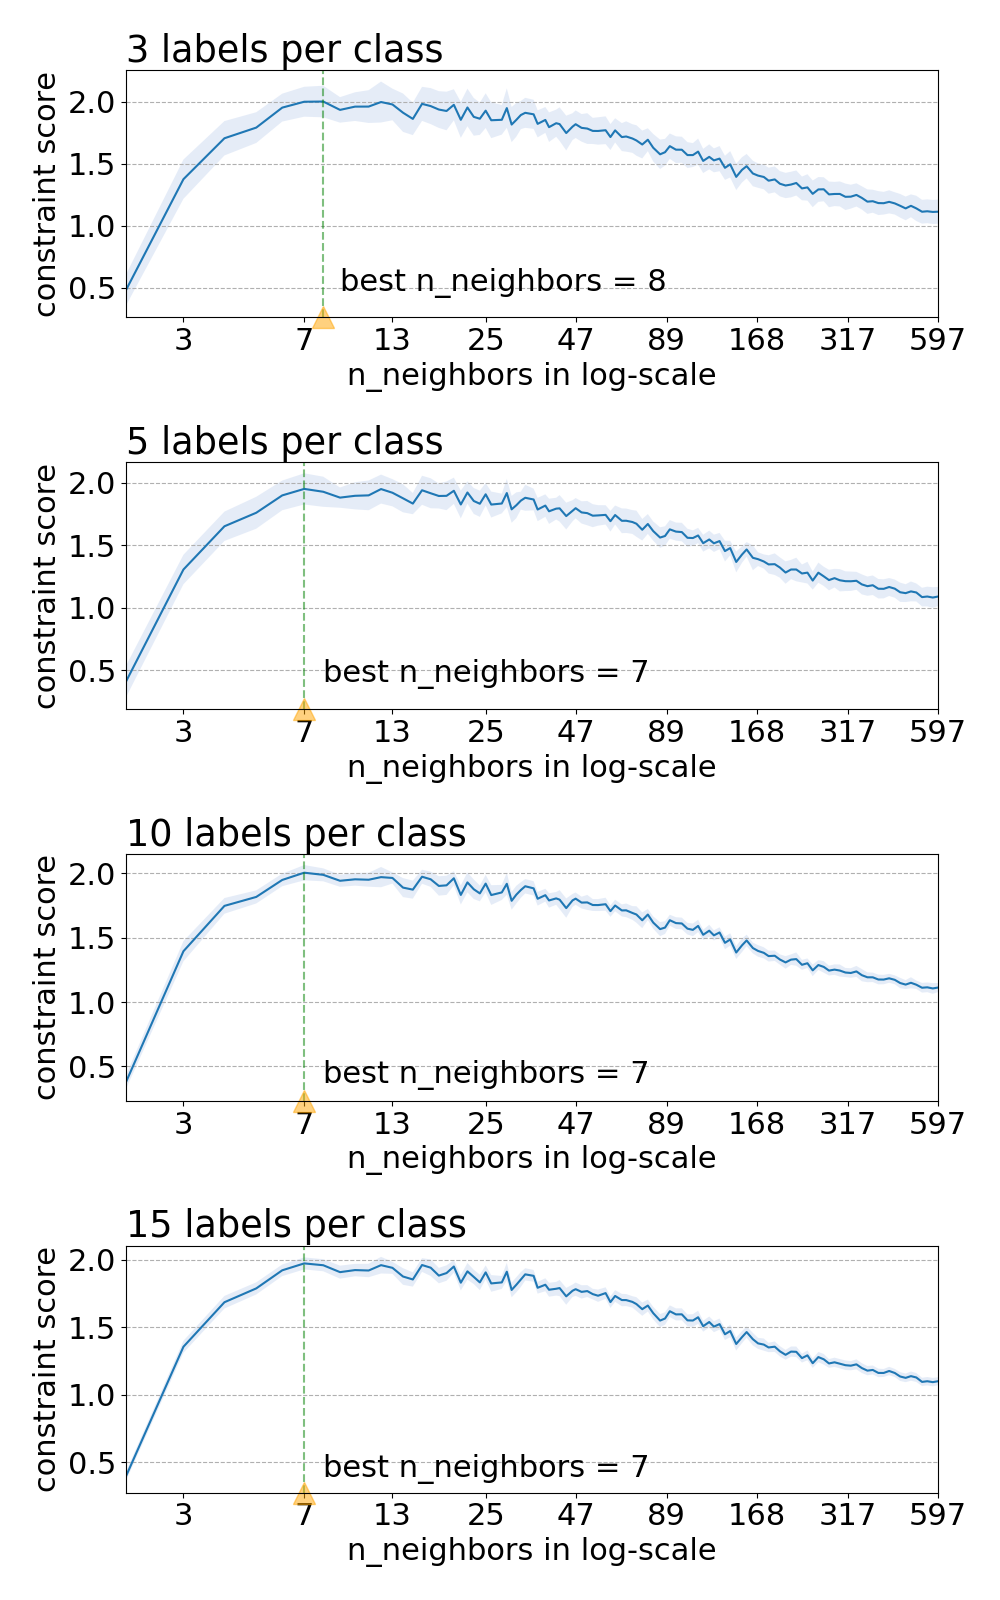
\includegraphics[width=\textwidth]{DIGITS_umap_scores}
         \caption{UMAP with DIGITS}
         \label{fig:s4}
     \end{subfigure}
     \hfill
     \begin{subfigure}[b]{0.32\textwidth}
         \centering
         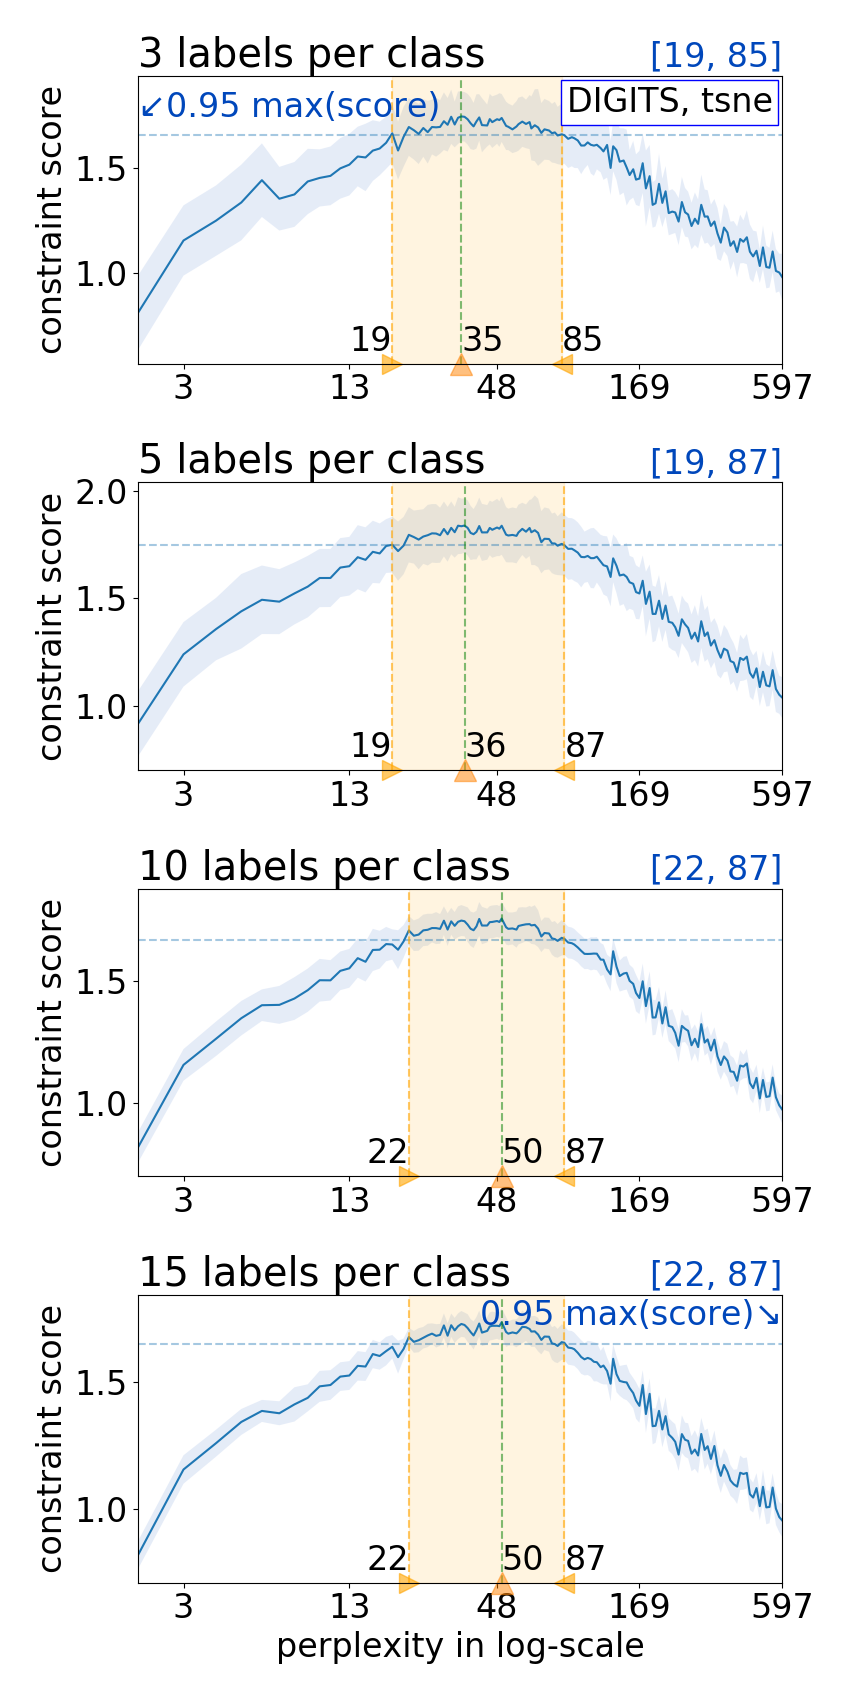
\includegraphics[width=\textwidth]{DIGITS_tsne_scores}
         \caption{t-SNE with DIGITS}
         \label{fig:s3}
     \end{subfigure}
     \hfill
     \begin{subfigure}[b]{0.32\textwidth}
         \centering
         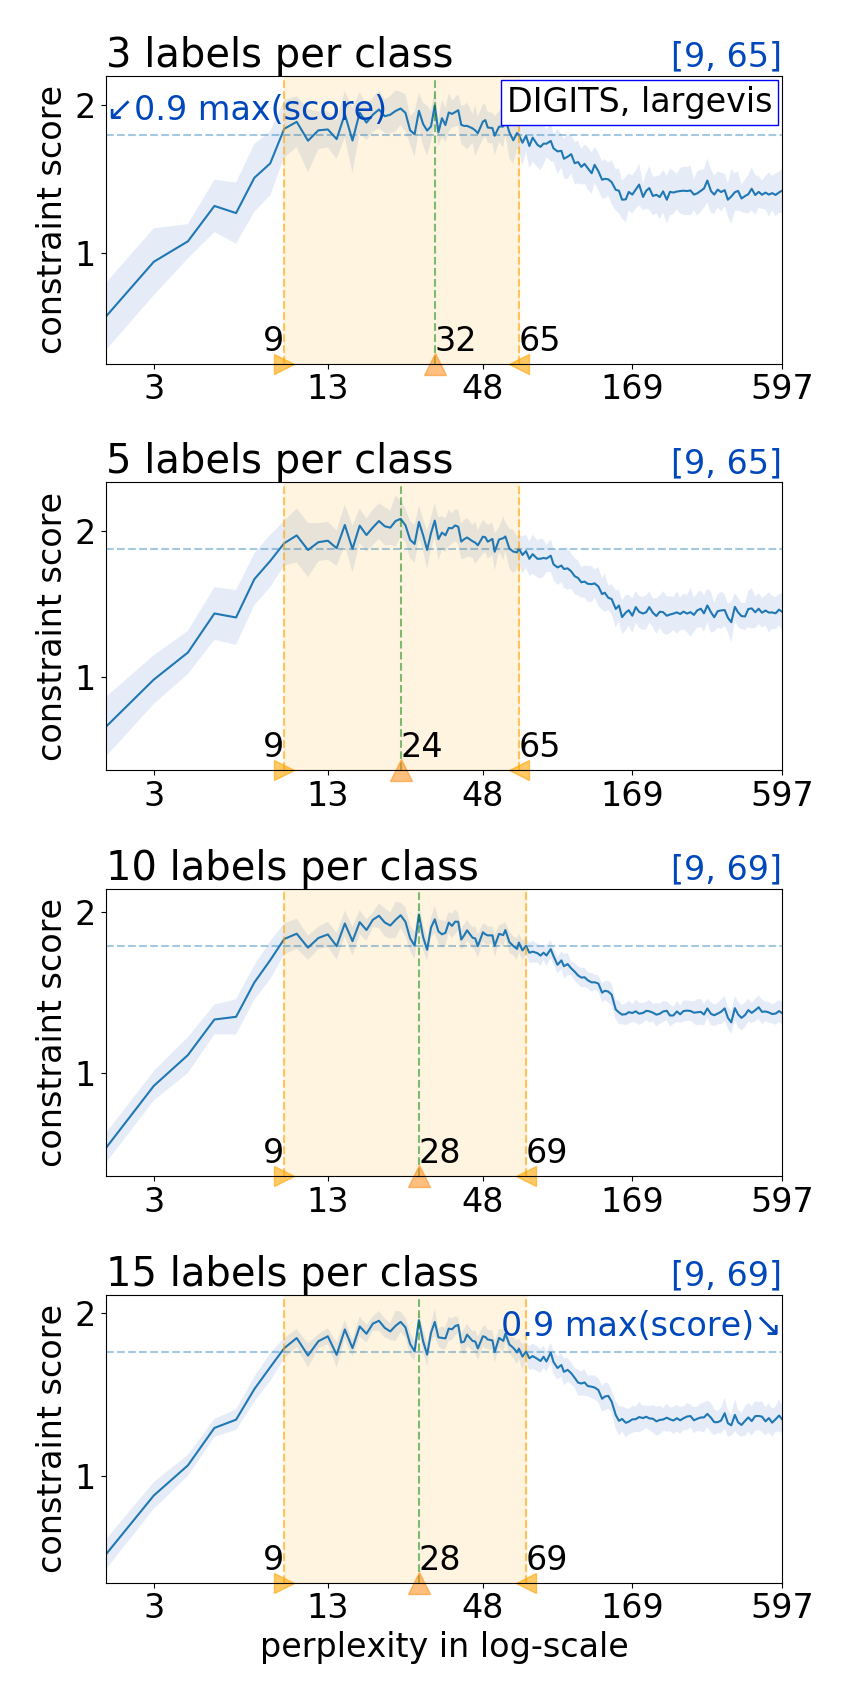
\includegraphics[width=\textwidth]{DIGITS_largevis_scores}
         \caption{LargeVis with DIGITS}
         \label{fig:s4}
     \end{subfigure}

     \caption{Stability of the constraint preserving scores with three methods UMAP, t-SNE and LargeVis for two datasets COIL20 and DIGITS}
     \label{fig:score_stability}
\end{figure*}


\vspace{8pt} \par
To discuss:

+ How to evaluate the visualization corresponding to the optimal hyperparam found by our method? => We can show this optimal viz and other `non-optimal' viz and analyze them visually/intuitively.

+ \st{Compare our score with John's score? (Apply BayOpt to John's metric, compare the predictive score function - the prediction line in the graphs, compare the optimal hyperparameter).}
(John's metric use HD data, time complexity of $O(DN^3)$ while our score is $O(DN^2)$ with a scale factor of the number of constraints.)

+ Compare our result with the method of auto-selecting perplexity of Cao and Wang? (TODO)





%%%%%%%%%%%%%%%%%%%%%%%%%%%%%%%%%%%%%%%%%%%%%%%%%%%%%%%%%%%%%%%%%%%
\section{Discussion}
Meeting 12/07: not sound enough for now, to discuss later.

\par
Discuss the variance of the proposed score (w.r.t to different set of constraints, different number of constraitns).
Say, the constraint-based score is a stochastic function.
Say, how BayOpt can take into account the uncertainty (the variance of the score) to estimate the maximum of this stochastic function.


\par
The violated constraints in our methods correspond to the shortcomming of t-SNE in \cite{wattenberg2016use}.
t-SNE can not preserve the within-cluster distances and between-clusters distances.
[TODO: Add reproduced figures].
The $q_{ij}$-based score can help to understand the defective of the visualization.
(E.g., can compare with google's embedding project, vis the neighbors in HD and LD, but it still hard to understand the model.
With our score, it is easier to visualize the violated constraints).

\par
Add discussion for UMAP.

\par
Easily generate pairwise constraints from labels.
  Only need small amount of labeled points for each class to generate hundreds of constraints.
  The proposed method only need 200 constraints to work well.
  [TODO: Test with smaller number of constraints to see if it works. 200 constraints seem too much].

\par
Can replace the auto-generated constraints by the manual constraints of the real user.

\par
The user can interact directly in the loop of Bayesian Optimization method to select the next hyperparameter to discover.


\par
Both the constraint-based score and the BayOpt's internal steps are explainable even for the non-technical users. 



%%%%%%%%%%%%%%%%%%%%%%%%%%%%%%%%%%%%%%%%%%%%%%%%%%%%%%%%%%%%%%%%%%%
\section{Conclusion and Future Work}

\par (1) Repeat the problem of hyperparameter tuning for DR methods and our solution:

+ The proposed constraint-based score is indenpendent to how the embedding is produced and can be used with any DR methods.
This score is built upon a limited number of constraints but can distinguish the visualizations prefering local structure and those prefereing global structure.

+ A finding that Bayesian Optimization approach fits well in our problem.


\vspace{8pt}
\par (2) Summary the advantages of the two above elements

+ The constraint-based score agree the the well-known quality metric.

+ This score can be visually represented to explain the violated pairs.

+ By combining this score with BayOpt approach, we can tune many hyperparameters at the same time for many widely used DR methods like t-SNE or UMAP.

+ BayOpt takes into account the uncertainty in the score values and also explainable. We can observe the internal optimization step to anwser the question: why to choose the next promissing hyperparameters to try?


\vspace{8pt}
\par (4) Future work:

(a) User experiment:

+ Integrate the user's feedback in two stages of our workflow.
The users can select the pairwise constraints or label some points (used to generate the constraints) to build the score.
They can also manualy select the next hyperparameters to evaluate in a customized interactive BayOpt framework.

+ Take the preference of the users on the presented visualizations to evaluate the quality of the visualization. We search for if the best visualization selected by the user corresponds to the result of our method.


(b) Integrate directly the pairwise constraints into the optimization process of BayOpt.
BayOpt is now used as a generic toolbox to find the extreme of a blackbox costly objective function.
Our idea is to use the pairwise constraint to modify the kernel in the covariance function of Gaussian Process model, which is the core element of BayOpt.
